\usetikzlibrary{arrows.meta}
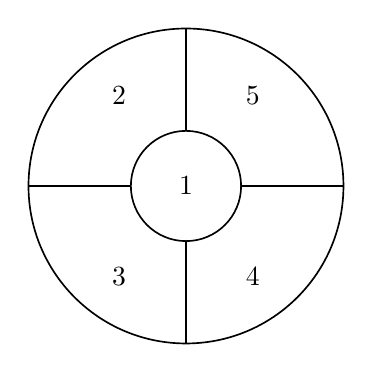
\begin{tikzpicture}[x=1cm,y=1cm,line width=.6pt,font=\normalsize]
\draw (0,0) circle[radius=2.0];
\draw (0,0) circle[radius=0.7];
\draw (0,0.7) -- (0,2.0);
\draw (0,-0.7) -- (0,-2.0);
\draw (-0.7,0) -- (-2.0,0);
\draw (0.7,0) -- (2.0,0);
\node[inner sep=0pt] at (0,0) {$1$};
\node[inner sep=0pt] at (-0.85,1.15) {$2$};
\node[inner sep=0pt] at (0.85,1.15) {$5$};
\node[inner sep=0pt] at (-0.85,-1.15) {$3$};
\node[inner sep=0pt] at (0.85,-1.15) {$4$};
\end{tikzpicture}
